% done
\part{Data analysis}
\label{part:data_analysis}

%------------------------------------

\section{About this part}
\label{section:DA_about_part}
Before rigorously testing different models available, it's important to take a look at the data that is supplied.
The supplied data consists of two main groups of images, labelled training images and unlabeled test images.
As per the requirements of the Kaggle competition, the test images should only be used for evaluating the model.
Thus the test images \textit{can not} be used for creating the model in any shape or form.
This means that only the labelled training images can be used to create and validate the model in development.
To avoid altering the model to perform well on the supplied test data and not in general, only the training data will be analysed.
Data leakage is also an important factor that will have to be taken into account when creating a further train and validation set from the training data.
All code used for this part is available under the developed code folder on GitHub, in the Jupyter Notebook \texttt{data\_analysis.ipynb}.
This part will only analyze the data and make suggestions for possible preprocessing, it won't manipulate the data just yet.
This notebook allows for changing parameters easily, which is crucial since this analysis has to be done for multiple descriptors and settings.

%------------------------------------

\section{Data distribution}
\label{section:DA_data_distribution}
The provided labeled training data consists of 12 different classes.
There is a total of 4042 labelled training images supplied, the distribution of which is shown in figure \ref{fig:1-data_analysis-labeled_data_distribution}.
As visible in this figure, the distribution between classes is not balanced.
This has to be taken into account when fitting a model since some models will show unwanted behaviour when fitted with unbalanced data.
Luckily many solutions exist to minify the impact of this unbalance.
This unbalance has to be kept in mind when using a split of the training data as a validation set as well.
This is because such split might lead to a test set where some classes have considerably fewer instances in the test set and thus the performance on those classes has less impact on the total score, which may be unwanted.

\begin{figure}[H]
    \centering
    \fbox{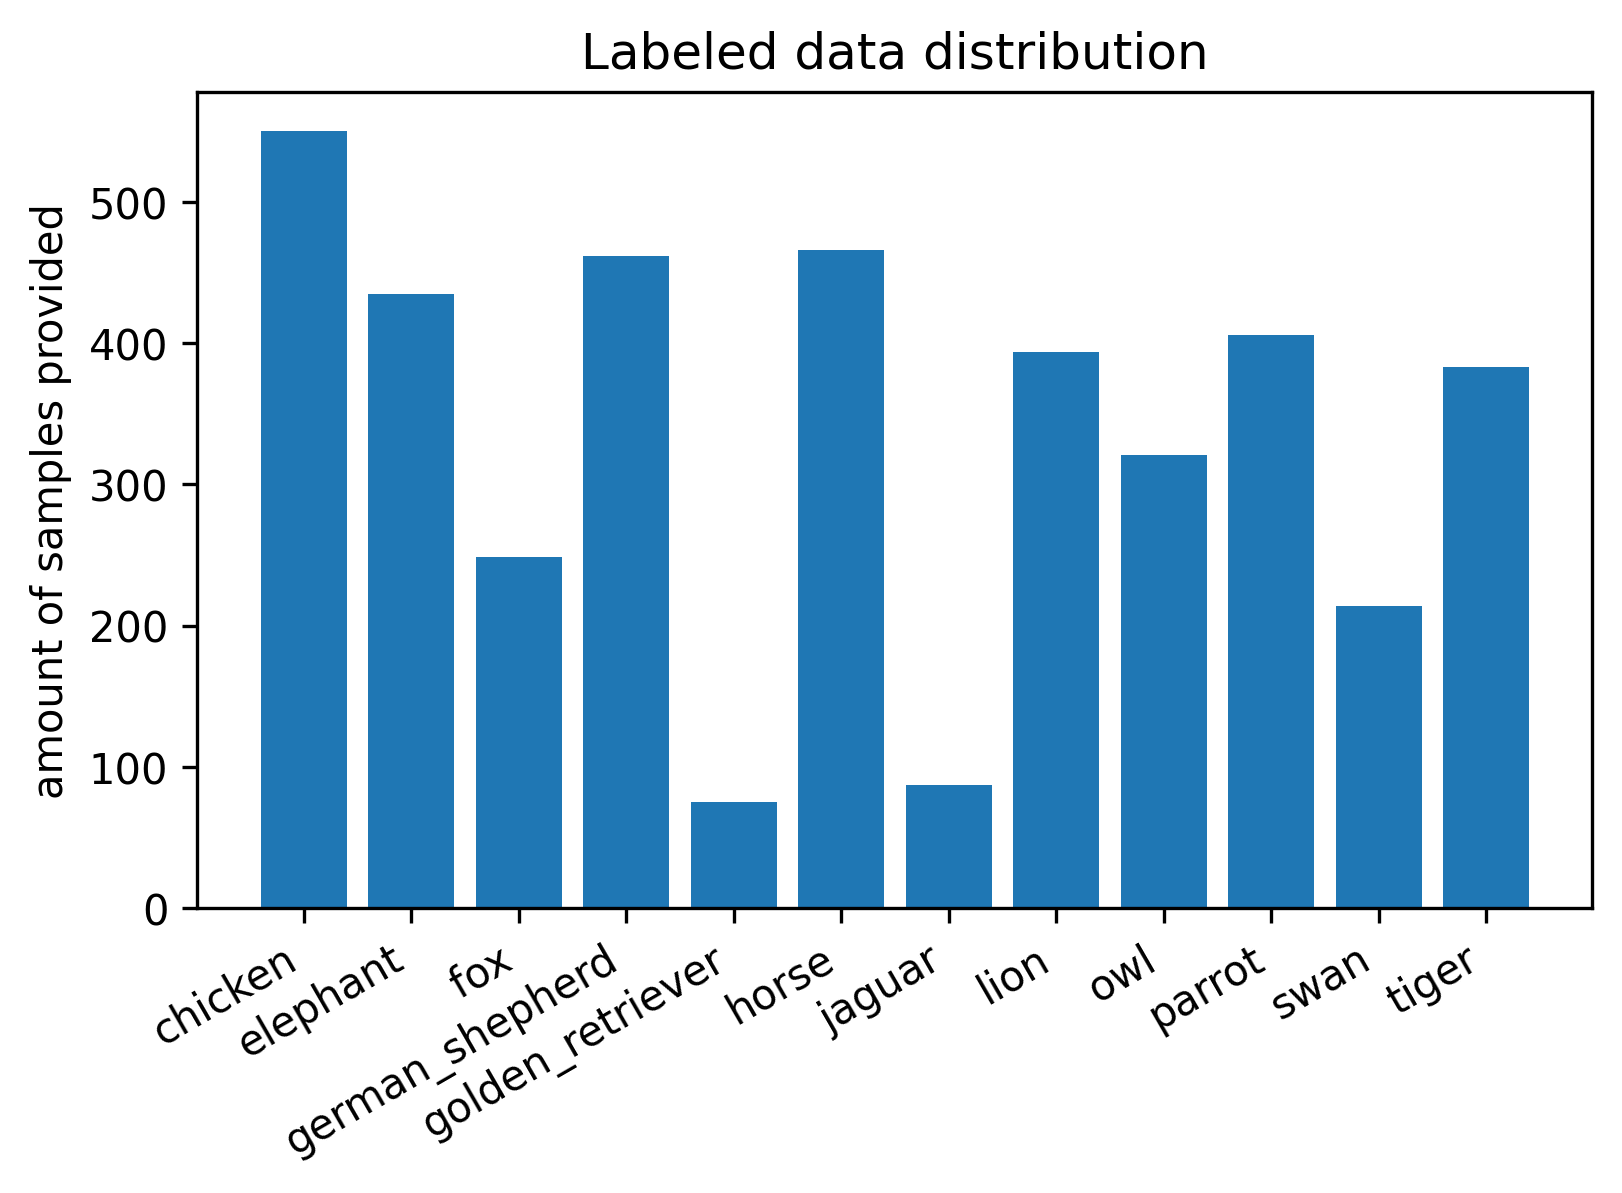
\includegraphics[width=0.55\linewidth]{images/1/1-data_analysis-labeled_data_distribution.png}}
    \captionsetup{width=0.5\linewidth}
    \captionsetup{justification=centering}
    \caption{Data distribution training data.}
    \label{fig:1-data_analysis-labeled_data_distribution}
\end{figure}

%------------------------------------

\section{Deeper look at the training data}
\label{section:DA_deeper_look_data}

Whilst noting that the available data isn't balanced over all the classes is very important, there are also different aspects of the data that need analysing. 
An overview of the supplied training data is given in figure \ref{fig:1-data_analysis-labeled_data_overview.png}, available in the figures list at the end of this report.
This figure shows the first five images of each class.
From this, it becomes apparent that multiple factors of the data aren't \emph{optimal}.
This knowledge is important since it can aid in better prepossessing and in finding a better model in general.
The most noteworthy findings are listed here:
\begin{itemize}
    \item Images vary in shapes, some are taken in portrait, others in landscape.
    \item Images vary in size, some are high resolution whilst others are relatively low resolution.
    \item The framing of the subject(s) varies a lot. Sometimes the labelled animal is completely visible and centred in the frame. In some images there are multiple animals spread across the image, others show a close-up of the animal.
    \item Some images have a detailed background that makes up for a lot of the image, in others the background is blurry and its impact is presumably less.
    \item Some images have very vibrant colours in broad daylight, others are black and white in dimly lit environments.
\end{itemize}

This diversity in the provided training set is expected since it has been scraped from the web.
This also means that \emph{noise} can be expected, another important factor to keep in mind when choosing and optimizing models.
Many of the listed things can be minified by doing some clever prepossessing of the images or are already taken into account by the used descriptor.


%------------------------------------

\section{Feature extraction and numerical representation}
\label{section:DA_feature_extraction_and_nr_rep}

Due to exclusive use of the supplied SIFT descriptor features for this report, information for this section is given as an appendix (appendix A).
The most important finding is the fact that the supplied \texttt{createCodebook} helper function uses \texttt{MiniBatchKMeans} for a given cluster amount, which can be fine-tuned.
More clusters will often result in better performance but gives the risk of overfitting.
It's also said the descriptor might benefit from fine-tuning as well, but this will not be done in this report, as will be discussed in part \ref{part:final_model}.

